\section{MPC feasibility}

\subsection{(a) Trajectories}

Fig. \ref{fig:mpc_traj} shows the closed and open loop trajectories for the system. 
%The black dashed curves are the open-loop trajectories predicted by MPC at each
%time step, while the colored curves show the realized closed-loop trajectory
%after applying only the first control from each solve. 
The orange trajectory starts from the larger velocity initial condition,
 so it is harder to slow down
because the input is bounded. Using \(P=P_{\mathrm{DARE}}\) gives a more useful
terminal cost than \(P=I\), since it approximates the infinite-horizon LQR
cost-to-go after the short MPC horizon. This makes the predicted plans
and the realized trajectory look more stabilizing and less short-sighted.

\begin{figure}[H]
\centering
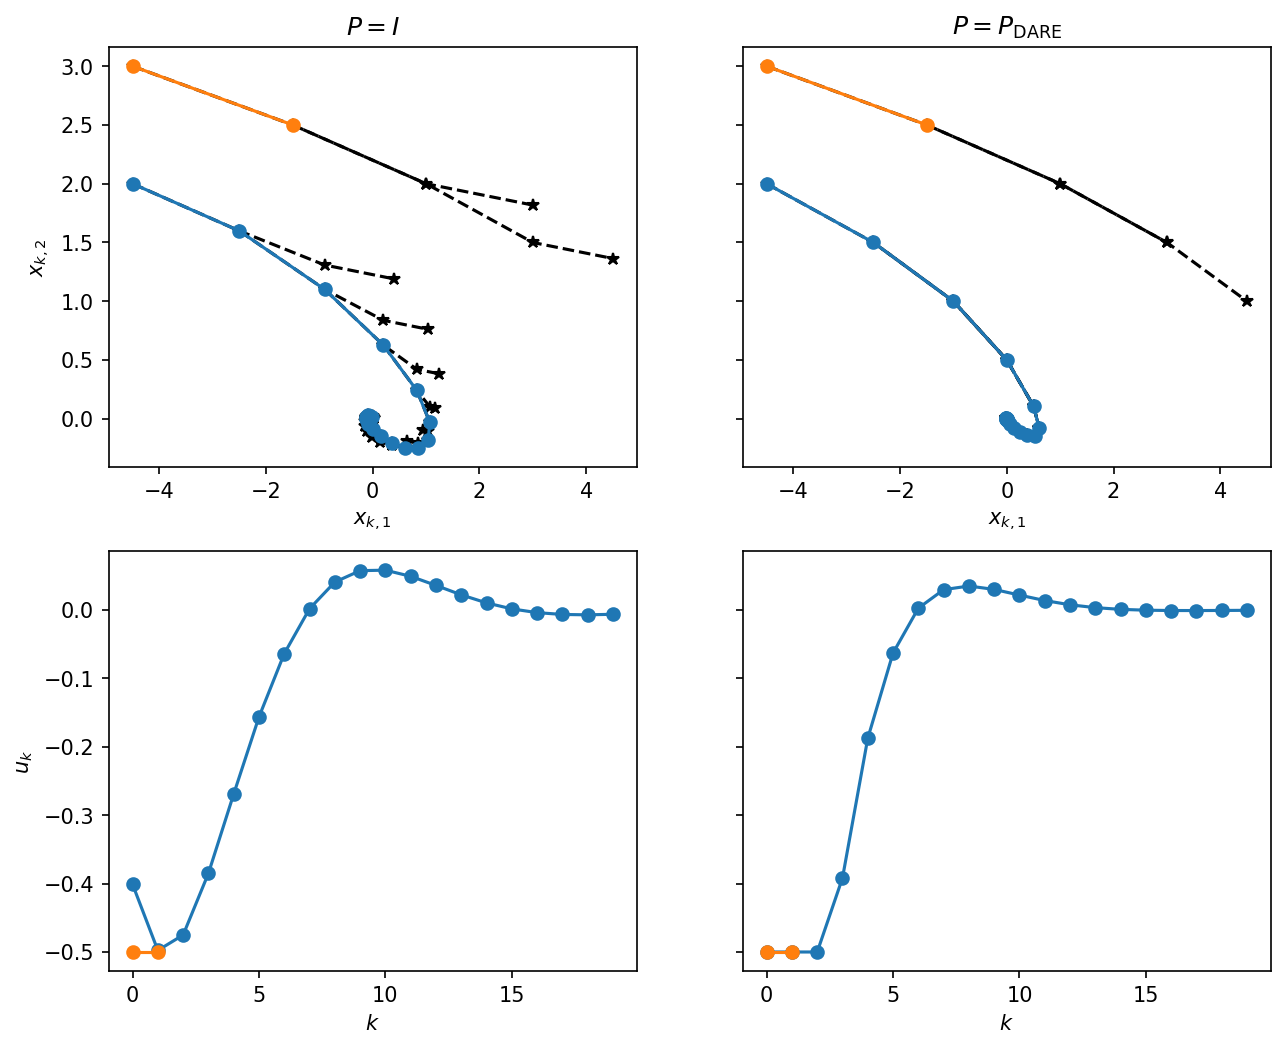
\includegraphics[width=0.5\textwidth]{figures/mpc_feasibility_sim.png}
\caption{Trajectories}
\label{fig:mpc_traj}
\end{figure}

\subsection{(b) Region of attraction}

Fig. \ref{fig:mpc_roa} shows the ROA obtained by simulating closed-loop MPC from
each grid point and marking the states that converge to the origin.
Longer horizons give a larger ROA because the controller can plan farther
ahead. The strict terminal constraint \(r_f=0\) makes the ROA smaller, while
\(r_f=\infty\) leaves feasibility mostly limited by the state and input bounds.

\begin{figure}[H]
\centering
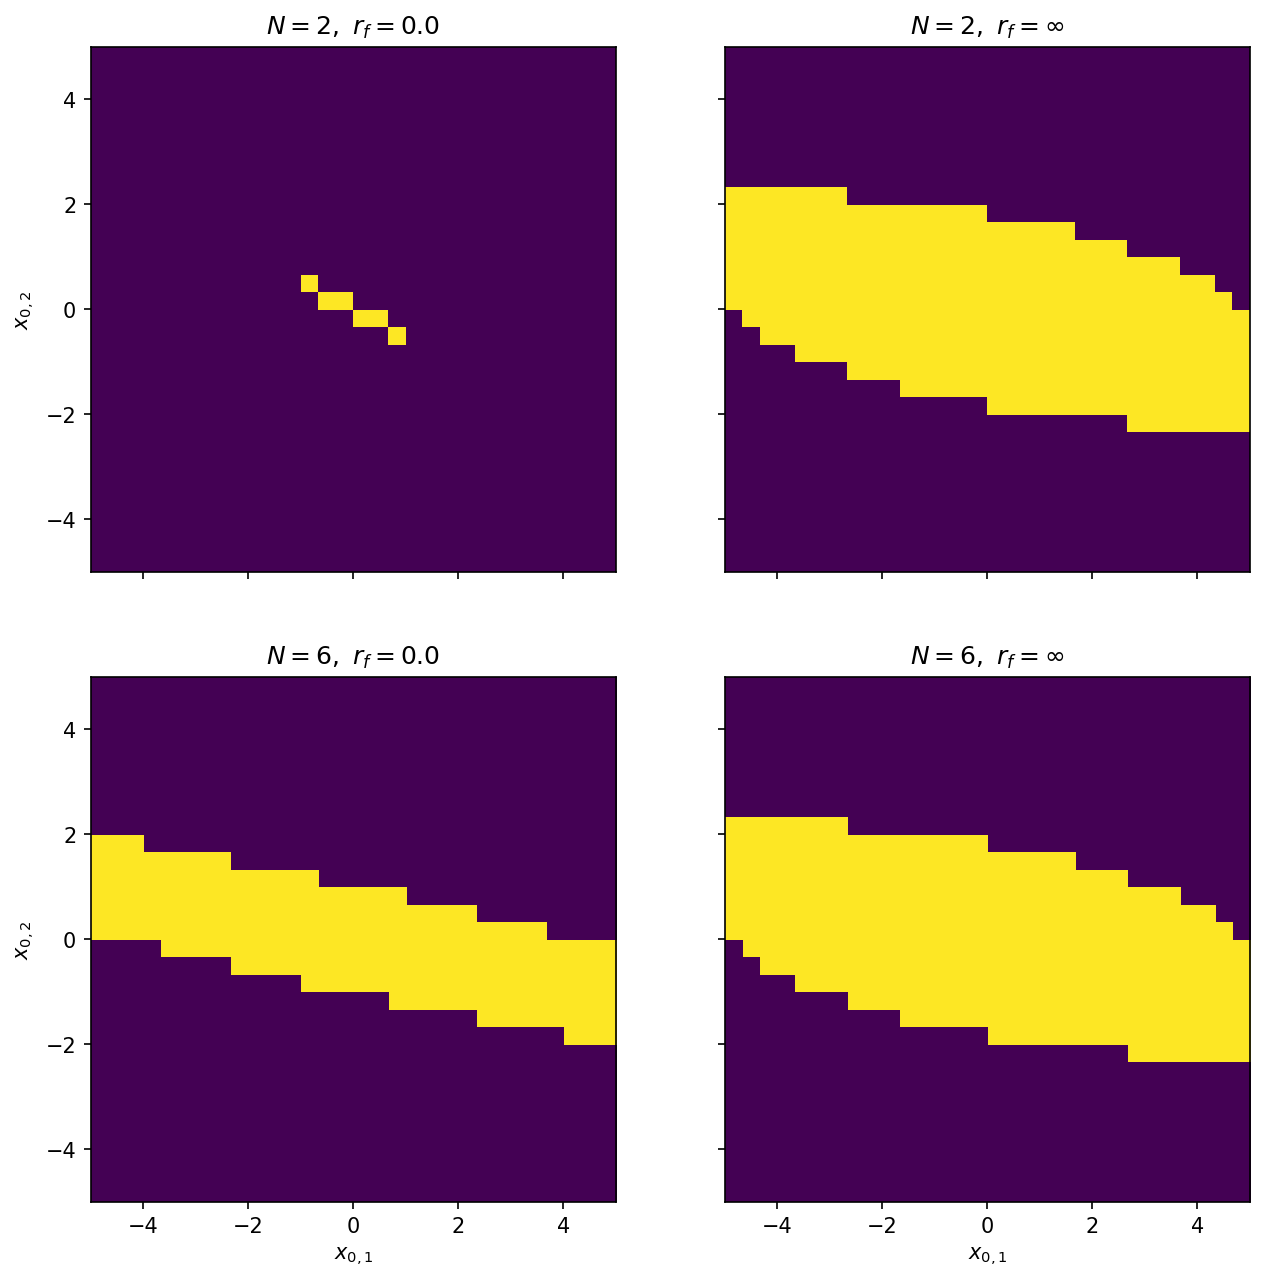
\includegraphics[width=0.7\textwidth]{figures/mpc_feasibility_roa.png}
\caption{Regions of attraction for different horizon lengths and terminal constraints}
\label{fig:mpc_roa}
\end{figure}

\subsection{Code}
Code in \hyperref[mpc_feasibility]{Appendix}.
